\documentclass{article}
\usepackage[utf8]{inputenc}
\usepackage{graphicx}
\usepackage{tikz}
\usepackage{amsmath, amsthm, amssymb}
\usepackage{geometry}
\usepackage{xcolor}
\geometry{a4paper, top=1in, bottom=1in, left=1in, right=1in}

\title{Practice Karls}
\author{Do Thanh Trung}
\date{\today}

\begin{document}

\maketitle

\section{Introduction}

This is a sample LaTeX article document. You can start writing your content here.

\section{TikZ Example}
The angle \textcolor{green}{$\alpha $ is $30^{\circ}$} in the example ($\pi/6$ in radians). The sine of $\alpha$, which is the height of the red line, is 
\begin{equation}
    \sin \alpha = 1/2.
\end{equation}
By the Theorem of Pythagoras we have $\cos^2 \alpha + \sin^2 \alpha = 1$. Thus the length of the blue line, which is the cosine of $\alpha$, must be
\begin{equation}
    \cos \alpha = \sqrt{1 - 1/4} = \frac{1}{2}\sqrt{3}.
\end{equation}
This shows that $\tan \alpha$, which is the height of the orange line, is
\begin{equation}
	\tan \alpha = \frac{\sin \alpha}{\cos \alpha} = \frac{1/2}{\sqrt{3}/2} = 1/\sqrt{3}.
\end{equation}
\begin{center}
	we are working on
	\begin{tikzpicture}
		\draw (-1.5,0) -- (1.5,0); % Draw x-axis
		\draw (0,-1.5) -- (0,1.5); %
	\end{tikzpicture}
	
	\tikz \draw (-1.5,0) -- (1.5,0) -- (0,-1.5) -- (0,1.5);
	
	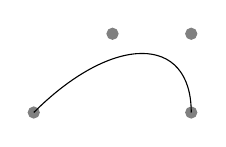
\begin{tikzpicture}
		\filldraw [gray] 	(0,0) circle [radius=2pt]
							(1,1) circle [radius=2pt]
							(2,1) circle [radius=2pt]
							(2,0) circle [radius=2pt];
		\draw (0,0) .. controls (1,1) and (2,1) .. (2,0);
	\end{tikzpicture}
	
	\begin{tikzpicture}
		\draw (-1.5,0) -- (1.5,0);
		\draw (0,-1.5) -- (0,1.5);
		\draw (-1,0) .. controls (-1,0.555) and (-0.555,1) .. (0,1)
					 .. controls (0.555, 1) and (1,0.555) .. (1,0);
	\end{tikzpicture}
\end{center}

\section{Circle Path Construction}
\begin{center}
	\tikz \draw (0,0) circle [radius=1cm];

	\tikz \draw (0,0) ellipse [x radius=1cm, y radius=0.5cm];

	\tikz \draw[rotate=30] (0,0) ellipse [x radius=1cm, y radius=0.5cm];

	\begin{tikzpicture}
		\draw (-1.5,0) -- (1.5,0);
		\draw (0,-1.5) -- (0,1.5);
		\draw (0,0) circle [radius=1cm];
	\end{tikzpicture}

\end{center}
\section{Rectangle Path Construction}
\begin{center}
	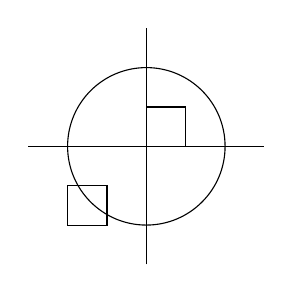
\begin{tikzpicture}
		\draw (-1.5,0) -- (1.5,0);
		\draw (0,-1.5) -- (0,1.5);
		\draw (0,0) circle [radius=1cm];
		\draw (0,0) rectangle (0.5,0.5);
		\draw (-0.5,-0.5) rectangle (-1,-1);
	\end{tikzpicture}
\end{center}

\section{Grid Path Construction}
\begin{center}
	\begin{tikzpicture}[scale=3]
		\draw (-1.5,0) -- (1.5,0);
		\draw (0,-1.5) -- (0,1.5);
		\draw (0,0) circle [radius=1cm];
		\draw[step=0.5cm,gray, very thin] (-1.4,-1.4) grid (1.4,1.4);
	\end{tikzpicture}
\end{center}

\section{Adding a Touch of Style}
\begin{center}
	\begin{tikzpicture}[scale=3]
		\tikzset{Karl's grid/.style ={help lines,color=#1!50},
			Karl's grid/.default=black}
		\draw[Karl's grid]	(0,0) grid (1.5,2);
		\draw[Karl's grid=red] (2,0) grid (3.5,2);
	\end{tikzpicture}
\end{center}

\end{document}